% begin module cycloid-tangents-ex2
\begin{frame}[t]
\begin{example} %[Example 2, p. 667]
Consider the cycloid $x = r(\theta - \sin \theta )$, $y = r(1 - \cos \theta )$.
\ 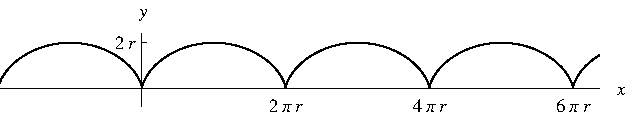
\includegraphics[height=1.5cm]{parametric-curves/pictures/11-02-ex2a.pdf}%
\begin{enumerate}
\item  At what points is the tangent horizontal?
\item  At what points is the tangent vertical?
\end{enumerate}
\end{example}
\end{frame}


\begin{frame}[t]
\begin{example} %[Example 2, p. 667]
Consider the cycloid \alert<handout:0| 5-6>{$x = r(\theta - \sin \theta )$}, \alert<handout:0| 3-4>{$y = r(1 - \cos \theta )$}.
\ \only<handout:0| -13>{%
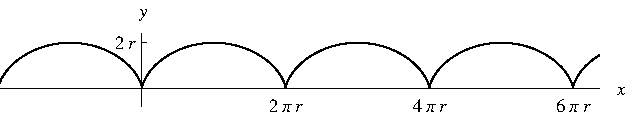
\includegraphics[height=1.5cm]{parametric-curves/pictures/11-02-ex2a.pdf}%
}%
\only<14->{%
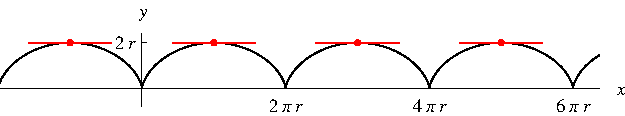
\includegraphics[height=1.5cm]{parametric-curves/pictures/11-02-ex2b.pdf}%
}%
\begin{enumerate}
\item  At what points is the tangent horizontal?
%\item  At what points is the tangent vertical?
\end{enumerate}
\begin{itemize}
\item<2->  The slope of the tangent is
\abovedisplayskip=0pt
\belowdisplayskip=0pt
\[
\uncover<2->{%
\frac{\diff y}{\diff x} = \frac{\alert<handout:0| 3-4>{\diff y /\diff \theta}}{\alert<handout:0| 5-6>{\diff x/\diff \theta}}%
}%
\uncover<3->{%
 = \frac{\alert<handout:0| 3-4>{\uncover<4->{r\sin \theta}}}{\alert<handout:0| 5-6>{\uncover<6->{r(1-\cos \theta )}}}%
}%
\uncover<7->{%
 = \frac{\sin \theta}{1-\cos \theta}%
}%
\]
\item<8->  The tangent is horizontal when $\diff y/\diff x = 0$, that is, when $\diff y/\diff \theta = 0$ and $\diff x/\diff \theta \neq 0$.
\item<9-| alert@10-11>  $r\sin\theta = \diff y/\diff \theta = 0$ if $\theta = $ \uncover<11->{$n\pi$, where $n$ is any integer.}
\item<9-| alert@12-13>  $r(1 - \cos\theta ) = \diff x/\diff \theta = 0$ if $\theta = $ \uncover<13->{$2n\pi$, where $n$ is any integer.}
\item<14->  Therefore there is a horizontal tangent when $\theta = (2n+1)\pi$.
\end{itemize}
\end{example}
\end{frame}



\begin{frame}[t]
\begin{example}[Example 2, p. 667]
Consider the cycloid $x = r(\theta - \sin \theta )$, $y = r(1 - \cos \theta )$.
\ \only<handout:0| -14>{%
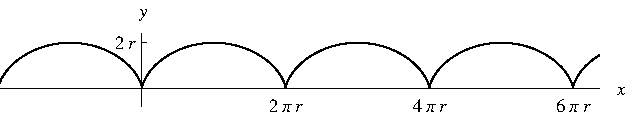
\includegraphics[height=1.5cm]{parametric-curves/pictures/11-02-ex2a.pdf}%
}%
\only<15->{%
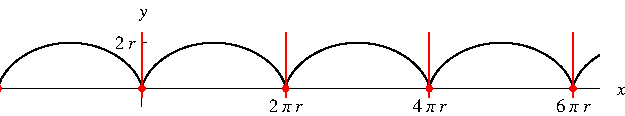
\includegraphics[height=1.5cm]{parametric-curves/pictures/11-02-ex2c.pdf}%
}%
\begin{enumerate}
\setcounter{enumi}{1}
%\item  At what points is the tangent horizontal?
\item  At what points is the tangent vertical?
\end{enumerate}
\begin{itemize}
\item<2->  When $\theta = 2n\pi$ both $\diff y/\diff \theta$ and $\diff x/\diff \theta$ are $0$.
\item<3->  To see if there is a vertical tangent, \alert<handout:0| 5-8>{use L'Hospital's Rule}.
\abovedisplayskip=0pt
\belowdisplayskip=0pt
\[
\uncover<4->{%
\lim_{\theta\to 2n\pi^+} \frac{\diff y}{\diff x} = \lim_{\theta\to 2n\pi^+} \frac{\alert<handout:0| 5-6>{\sin \theta}}{\alert<handout:0| 7-8>{1-\cos \theta}}%
}%
\uncover<5->{%
 = \lim_{\theta\to 2n\pi^+} \frac{\alert<handout:0| 5-6,9-10>{\uncover<6->{\cos \theta}}}{\alert<handout:0| 7-8,11-12>{\uncover<8->{\sin \theta}}}%
}%
\uncover<9->{%
{%
\uncover<9->{\alert<handout:0| 9-10>{\to}} \atop%
\uncover<11->{\alert<handout:0| 11-12>{\to}} }%
\frac{\uncover<10->{\alert<handout:0| 9-10>{1}}}{\uncover<12->{\alert<handout:0| 11-12>{0^+}}} %
}%
\]
\item<13->  Therefore $\lim_{\theta\to 2n\pi^+} (\diff y/\diff x) = \infty$.
\item<14->  A similar argument shows $\lim_{\theta\to 2n\pi^-} (\diff y/\diff x) = -\infty$.
\item<15->  Therefore there is a vertical tangent when $\theta = 2n\pi$.
\end{itemize}
\end{example}
\end{frame}
% end module cycloid-tangents-ex2
